\documentclass[12pt,a4paper]{article}
\usepackage[T2A]{fontenc}
\usepackage[utf8]{inputenc}
\usepackage[russian]{babel}
\usepackage{amsmath}
\usepackage{amssymb}
\usepackage{graphicx}
\usepackage{floatrow}
\usepackage{booktabs}
\usepackage{wrapfig}
\usepackage{lipsum}
\usepackage{subcaption}
\usepackage{wrapfig,lipsum,booktabs}

\newcommand{\figref}[1]{(См. рис. \ref{#1})}
\newcommand{\secref}[1]{(См. раздел. \ref{#1})}

\newcommand{\e}[1]{\text{$\cdot10^{#1}$}}

\newcommand{\uu}[1]{\text{$\text{#1}$}}
\newcommand{\uf}[2]{\text{$\frac{\text{#1}}{\text{#2}}$}}

\newcommand{\tabname}[2]{
	\toprule
	\multicolumn{#1}{c}{\text{#2}} \\
	\toprule
}


\author{\normalsize Выполнил: Дедков Денис, группа Б01-109 \\
	\normalsize 14.03.2022}
\date{}



\usepackage{float}
\restylefloat{table}
\title
{
	\large Отчет о выполнении лабораторной работы 1.3.3 \\
	\Large Определение вязкости воздуха по скорости течения через тонкие трубки \\ 
}


\begin{document}
	\maketitle
	
	\subsection*{Цель работы} Экспериментально выявить участок сформированного течения, определить режимы ламинарного и турбулентного течения; определить число Рейнольдса.
	
	\subsection*{Теоретическое введение}
	Рассмотрим движение вязкой жидкости или газа по трубке круглого сечения. При малых скоростях потока движение оказывается ламинарным (слоистым), скорости частиц меняются по радиусу и направлены вдоль оси трубки. С увеличением скорости потока движение становится турбулентным, и слои перемешиваются. При турбулентном движении скорость в каждой точке быстро меняет величину и направление, сохраняется только средняя величина скорости.
	Характер движения газа (или жидкости) в трубке определяется безразмерным числом Рейнольдса:
	
	\begin{equation}
		Re = \dfrac{\upsilon r \rho}{\eta}
	\end{equation}
	
	где $\upsilon$ - скорость потока, $r$ - радиус трубки, $\rho$ - плотность движущейся среды, $\eta$ - вязкость. В гладких трубах круглого сечения переход от ламинарного движения к турбулентному происходит при $Re \approx 1000$
	
	При ламинарном течении объем газа $V$, протекающий за время $t$ по трубе длиной $l$, определяется формулой Пуазейля:
	
	\begin{equation} \label{form:QP}
		Q = \dfrac{\pi r^4}{8 l \eta}(P_1 - P_2)
	\end{equation}

	В этой формуле $P_1 - P_2$ - разность давлений в двух выбранных сечениях 1 и 2, расстояние между которыми равно $l$. Велечину $Q$ обычно называют расходом. Формула (2) позволяет определять вязкость газа по его расходу.
	
	Отметим условия, при которых справедлива формула (2). Прежде всего необходимо, чтобы с достаточным запасом выполнялось неравенство $Re < 1000$. Необходимо также, чтобы при течении не происходило существенного изменения удельного объема газа (при выводе формулы удельный объем считался постоянным). Для жидкости это предположение выполняется практически всегда, а для газа - лишь в тех случаях, когда перепад давлений вдоль трубки мал по сравнению с самим давлением. В нашем случае давление газа равно атмосферному ($10^3$ см вод. ст.), а перепад давлений составляет не более 10 см вод. ст., то есть менее $1\%$ от атмосферного. Формула (2) выводится для участков трубки, на которых закон распределения скоростей газа по сечению не меняется при движении вдоль потока.
	
	\begin{figure}[H]
		\begin{center}
			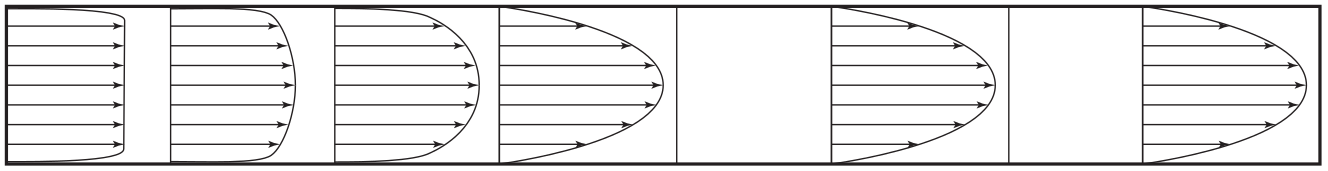
\includegraphics[width=12cm]{res/potok.png}
		\end{center}
		\caption{Формирование потока газа в трубе круглого сечения}
		\label{img1}
	\end{figure}	
	
	
	При втекании газа в трубку из большого резервуара скорости слоев вначале постоянны по всему сечению (рис. 1). По мере продвижения газа по трубке картина распределения скоростей меняется, так как сила трения о стенку тормозит прилежащие к ней слои. Характерное для ламинарного течения параболическое распределение скоростей устанавливается на некотором расстоянии $a$ от входа в трубку, которое зависит от радиуса трубки $r$ и числа Рейнольдса по формуле
	
	\begin{equation}
		a \approx  0,2 r \cdot Re
	\end{equation}

	Градиент давления на участке формирования потока оказывается большим, чем на участке с установившимся ламинарным течением, что позволяет разделить эти участки экспериментально. Формула (3) дает возможность оценить длину участка формирования.
	\subsection*{Экспериментальная установка}
	
	\begin{figure}[H]
		\begin{center}
			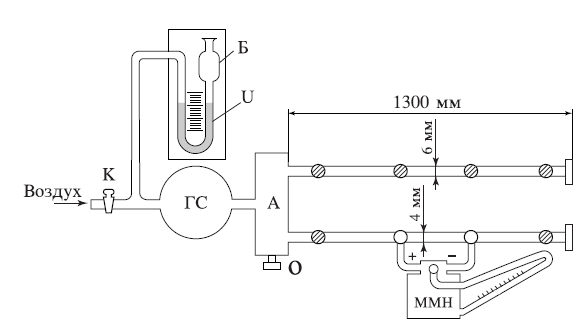
\includegraphics[width=12cm]{res/scheme.png}
		\end{center}
		\caption{Схема установки для определения вязкости воздуха}
		\label{img2}
	\end{figure}	
	
	Измерения производятся на экспериментальной установке, схема которой изображена на рис. 2. Поток воздуха под давлением, несколько превышающим атмосферное (на 5-7 см вод. ст.), через газовый счетчик ГС поступает в резервуар А, к которому припаяны тонкие металлические трубки. Примерные размеры трубок указаны на рисунке (точные размеры обозначены на установке). Обе трубки на концах снабжены заглушками, не пропускающими воздух. Во время измерений заглушка открывается только на рабочей трубке; конец другой трубки должен быть плотно закрыт. Перед входом в газосчётчик поставлена U-образная трубка, наполовину заполненная водой. Она выполняет две задачи. Первая - измерение давления газа на входе в газосчётчик. Вторая - предохранение газосчётчика от выхода из строя. Дело в том, что газосчётчик устойчиво работает, если давление газа на его входе не превышает 600 мм водяного столба. Высота U-образной трубки примерно 600 мм, поэтому, когда давление на входе в счётчик превышает 600 мм водяного столба,вода из U-образной трубки выплёскивается в защитный баллон Б и, создавая шум, привлекает к себе внимание экспериментатора. 


\subsection*{Ход работы}



Данные эксперимента $Q(P)$ занесем в таблицу \ref{tab:QP}. Построим графики зависимостей для качественного анализа поведения $Q(P)$ (см. рис. \ref{fig:QP}).
Из графиков четко видно, с какого момента начинается турбулентное течение. Через соответствующие линейные участки, где наблюдается ламинарное течение, проведены прямые.

Расчет вязкости проведем по формуле, прямо вытекающей из \ref{form:QP}. Она имеет следующий вид:
$$\eta = \frac{\pi R^4}{8la},$$
где $a$ - коэффициент наклона графика $Q(P)$.
Статистическая обработка проведена \textbf{методом наименьших квадратов} и занесена в таблицу \ref{tab:ab}.
Рассчитаем число Рейнольдса по следующей формуле:
$$Re_{\text{кр}} = \frac{\rho Q_{\text{кр}}}{\pi R \eta},$$
где параметры взяты из графика. Соответствующие значения занесем в таблицу \ref{tab:ab}.

Для определения соответствия теории и эксперимента проведем сравнение экспериментально найденной длины установления и теоретически определенной по следующей формуле:
$$l_{\text{уст}} \approx  0,2 r \cdot Re.$$

Для этого построим график (см. рис. \ref{fig:PX}) по данным таблицы \ref{tab:PX}, а также проведем вычисления по приведенной выше формуле. Расчеты занесем в таблицу \ref{tab:PXS}.

Для проверки формулы Пуазёйля проведем линеаризацию $\ln{\frac{Q \eta l}{P}} (\ln{R})$ (см. таблицу \ref{tablnlne}). График зависимости приведен на рисунке \ref{fig:lnln}. Расчет показателя степени сделан методом наименьших квадратов. Вся статистическая обработка занесена в таблицу \ref{tablll}.

\subsubsection*{Метод наименьших квадратов}
Перейдем к расчету зависимостей. Обработку проведем методом наименьших квадратов:

$$y = ax + b,$$

где $$a = \frac{r_{xy}}{ \sigma_x^2},$$
$$b = \overline{y} - a\overline{x}.$$

Для оценки погрешностей используем следующие формулы:
$$\sigma_a =  t_{n-1, p} \sqrt{\frac{1}{n-2} \left( \frac{\sigma_y^2}{\sigma_x^2} - A^2 \right)},$$
$$\sigma_b = \sigma_a \sqrt{\sigma_x^2 + \overline{x}^2},$$
где 
$n$ - количество измерений, $ t_{n-1, p}$ - коэффициент Стьюдента

Для определения расстояния
\begin{table}[H]
	
	\caption{Обработка для $Q(P)$}
	\label{tab:ab}
	\centering
	\footnotesize
	\begin{tabular}{lccccccc}
		\toprule
		
		Трубка & $a$ & $\sigma_a$ & $b$ & $\sigma_b$ & $\eta \pm \sigma_{\eta}$ & $Q_{\text{кр}}, \uf{л}{с}$ & $Re_{\text{кр}}$\\
		\midrule
		3 мм & 0.000341  &  0.000009 & 0.000986    & 0.000719 & $(1.94\pm0.09)\e{-5}$ & 0.05 & 656\\ 
		4 мм & 0.00061   &  0.00001  & -0.001108   & 0.00074  & $(1.96\pm0.09)\e{-5}$ & 0.07 & 691\\ 
		5 мм & 0.002046  &  0.000035 & -0.001798   & 0.001315 & $(1.62\pm0.08)\e{-5}$ & 0.12 & 1110\\ 
		\bottomrule
	\end{tabular}
\end{table}

\begin{table}[H]
	
	\caption{Обработка для  $\ln{\frac{Q \eta l}{P}} (\ln{R})$}
	\label{tablll}
	\centering
	\footnotesize
	\begin{tabular}{lcccc}
		\toprule
		$a$ & $\sigma_a$ & $b$ & $\sigma_b$ & $n\pm\sigma_n$\\
		\midrule
		3.814021  &  0.046102 & 2.162223  &  0.258724 & $(3.8\pm 0.05)$ \\
		\bottomrule
	\end{tabular}
\end{table}

\begin{figure}[H]
	\centering
	\includegraphics[width=1\linewidth]{"QdP"}
	\caption{Расход от давления}
	\label{fig:QP}
\end{figure}

\begin{figure}[H]
	\centering
	\includegraphics[width=1\linewidth]{"LN"}
	\caption{Линеаризация}
	\label{fig:lnln}
\end{figure}


\begin{table}[H]
	\caption{Расход от давления}
	\label{tab:QP}
	\begin{tabular}[t]{cccc}
		\tabname{4}{Трубка 3 мм}
		$t$, с & $\Delta V,\uu{л}$  & $Q,\uf{л}{c}$ & $P,\uu{Па} $ \\
		\midrule
		28.52 & 0.10 & 0.0035 & 9.74 \\
15.11 & 0.10 & 0.0066 & 19.48 \\
17.89 & 0.20 & 0.0112 & 29.22 \\
13.57 & 0.20 & 0.0147 & 38.96 \\
11.15 & 0.20 & 0.0179 & 48.70 \\
9.28 & 0.20 & 0.0216 & 58.44 \\
12.40 & 0.30 & 0.0242 & 68.18 \\
10.72 & 0.30 & 0.0280 & 77.92 \\
10.04 & 0.30 & 0.0299 & 87.66 \\
11.11 & 0.40 & 0.0360 & 97.40 \\
9.45 & 0.40 & 0.0423 & 116.88 \\
11.11 & 0.50 & 0.0450 & 136.36 \\
10.55 & 0.50 & 0.0474 & 155.84 \\
9.20 & 0.50 & 0.0543 & 175.32 \\
8.90 & 0.50 & 0.0562 & 194.80 \\
11.12 & 0.40 & 0.0360 & 107.14 \\
11.18 & 0.50 & 0.0447 & 126.62 
		\\\bottomrule
	\end{tabular}
	\hfill
	\begin{tabular}[t]{cccc}
		\tabname{4}{Трубка 4 мм}
		$t$, с & $\Delta V,\uu{л}$  & $Q,\uf{л}{c}$ & $P,\uu{Па} $ \\
		\midrule
		54.76 & 0.50 & 0.0091 & 17.53 \\
22.10 & 0.50 & 0.0226 & 38.96 \\
28.61 & 1.00 & 0.0350 & 58.44 \\
21.08 & 1.00 & 0.0474 & 77.92 \\
17.48 & 1.00 & 0.0572 & 97.40 \\
14.25 & 1.00 & 0.0702 & 116.88 \\
18.68 & 1.50 & 0.0803 & 136.36 \\
22.72 & 2.00 & 0.0880 & 155.84 \\
20.41 & 2.00 & 0.0980 & 175.32 \\
19.01 & 2.00 & 0.1052 & 194.80 \\
18.98 & 2.00 & 0.1054 & 214.28 \\
18.40 & 2.00 & 0.1087 & 253.24 \\
17.13 & 2.00 & 0.1168 & 292.20 \\
16.48 & 2.00 & 0.1214 & 331.16 \\
29.00 & 0.50 & 0.0172 & 29.22 \\
18.00 & 0.50 & 0.0278 & 48.70 \\
12.40 & 0.50 & 0.0403 & 68.18 \\
9.76 & 0.50 & 0.0512 & 87.66 \\
7.95 & 0.50 & 0.0629 & 107.14 \\
6.56 & 0.50 & 0.0762 & 126.62 \\
5.89 & 0.50 & 0.0849 & 146.10 
		\\\bottomrule
	\end{tabular}
	
	\begin{tabular}[LEFT]{cccc}
		\tabname{4}{Трубка 5 мм}
		$t$, с & $\Delta V,\uu{л}$  & $Q,\uf{л}{c}$ & $P,\uu{Па} $ \\
		\midrule
		12.90 & 0.50 & 0.0388 & 19.48 \\
8.83 & 0.50 & 0.0566 & 29.22 \\
12.66 & 1.00 & 0.0790 & 38.96 \\
10.41 & 1.00 & 0.0961 & 48.70 \\
8.41 & 1.00 & 0.1189 & 58.44 \\
8.04 & 1.00 & 0.1244 & 68.18 \\
7.27 & 1.00 & 0.1376 & 77.92 \\
6.71 & 1.00 & 0.1490 & 87.66 \\
10.08 & 1.50 & 0.1488 & 97.40 \\
10.01 & 1.50 & 0.1499 & 107.14 \\
9.69 & 1.50 & 0.1548 & 116.88 \\
27.34 & 0.50 & 0.0183 & 9.74 
		\\\bottomrule
	\end{tabular}
	\hfill
	\begin{tabular}[t]{cccc}
	\end{tabular}
\end{table}	




\begin{figure}[H]
	\centering
	\includegraphics[width=1\linewidth]{"PX"}
	\caption{Давление от координаты}
	\label{fig:PX}
\end{figure}


\begin{table}[H]
	\caption{Давление от координаты}
	\label{tab:PX}
	\begin{tabular}[t]{cc}
		\tabname{2}{Трубка 3 мм}
		$x, \uu{см}$ &  $P,\uu{Па} $ \\
		\midrule
		11.00 & 105.19 \\
31.00 & 187.01 \\
61.00 & 284.41 
		\\\bottomrule
	\end{tabular}
\hfill
	\begin{tabular}[t]{cc}
		\tabname{2}{Трубка 4 мм}
		$x, \uu{см}$ &  $P,\uu{Па} $ \\
		\midrule
		10.90 & 77.92 \\
40.90 & 165.58 \\
80.90 & 280.51 \\
130.90 & 408.11 
		\\\bottomrule
	\end{tabular}
\hfill
	\begin{tabular}[t]{cc}
		\tabname{2}{Трубка 5 мм}
		$x, \uu{см}$ &  $P,\uu{Па} $ \\
		\midrule
		10.70 & 50.65 \\
40.70 & 89.61 \\
80.70 & 128.57 \\
130.70 & 177.27 
		\\\bottomrule
	\end{tabular}
\end{table}	


\begin{table}[H]
	
	\caption{Линеаризация $\ln{\frac{Q \eta l}{P}} (\ln{R})$}
	\centering
	\footnotesize
	\label{tablnlne}
	\begin{tabular}[t]{cc}
		\toprule
		$\ln{R}$, с & $\ln{\frac{Q \eta l}{P}}$ \\
		\midrule
		-5.809 & -19.983 \\
-5.809 & -20.041 \\
-5.809 & -19.922 \\
-5.809 & -19.933 \\
-5.809 & -19.960 \\
-5.809 & -19.959 \\
-5.809 & -19.997 \\
-5.809 & -19.985 \\
-5.809 & -20.037 \\
-5.809 & -19.956 \\
-5.809 & -19.977 \\
-5.809 & -20.070 \\
-5.534 & -19.094 \\
-5.534 & -18.985 \\
-5.534 & -18.955 \\
-5.534 & -18.937 \\
-5.534 & -18.973 \\
-5.534 & -18.951 \\
-5.279 & -17.942 \\
-5.279 & -17.968 \\
-5.279 & -17.923 \\
-5.279 & -17.951 \\
-5.279 & -17.919 \\
-5.279 & -18.000 
		\\\bottomrule
	\end{tabular}
\end{table}

\clearpage
\subsection*{Вывод}
В ходе работы были экспериментально выявлены участки ламинарного и турбулентного течения воздуха при прохождении через круглые трубки. Легко увидеть (см. таблицу \ref{tab:PXS}), что эксперимент неплохо соответствует теории.

\begin{table}[H]
	
	\caption{Длина установления}
	\label{tab:PXS}
	\centering
	\footnotesize
	\begin{tabular}{lcccc}
		\toprule
		Трубка & Длина установления (теория), см & Длина установления (эксперимент), см \\
		\midrule
		3 мм & 20  &  20-25 \\
		4 мм & 30  &  35-40 \\
		5 мм & 56  &  30-45 \\
		\bottomrule
	\end{tabular}
\end{table}

Также была определена вязкость воздуха и число Рейнольдса (см. таблицу \ref{tab:vivod}).
Заметно, что значения при диаметрах трубок 3 мм и 4 мм немного отличаются от значения, полученного на трубке диаметра 5 мм.
\begin{table}[H]
	\caption{Вывод}
	\label{tab:vivod}
	\centering
	\footnotesize
	\begin{tabular}{lccccccc}
		\toprule
		
		$$ & $\eta \pm \sigma_{\eta}, \uf{кг}{м с}$ & $Re_{\text{кр}}$\\
		\midrule
		Трубка 3 мм &  $(1.94\pm0.09)\e{-5}$ & 656\\ 
		Трубка 4 мм &  $(1.96\pm0.09)\e{-5}$ &  691\\ 
		Трубка 5 мм & $(1.62\pm0.08)\e{-5}$ &  1110\\ 
		Табличное & $1.8\e{-5}$ &  800-1000\\
		\bottomrule
	\end{tabular}
\end{table}

Также был определен показатель степени в формуле Пуазёйля, который не сильно отличается от теории (доверительная вероятность $65\%$):
$$n_{\text{эксперимент}} = (3.8\pm 0.05)$$
$$n_{\text{теория}} = 4$$
\end{document}